\documentclass[12]{amsart}

\usepackage{amssymb,amsmath}

%\usepackage{refcheck}

\usepackage{graphicx}
\usepackage{amssymb}
\usepackage{mathrsfs}
\usepackage{amsmath}
\usepackage{latexsym}
\usepackage{amssymb}
\usepackage{enumerate}
\usepackage{fullpage} 
\usepackage{setspace}
\usepackage{color}
%\usepackage{ dsfont }
\usepackage{float}
\usepackage{physics}

%new math symbols taking no arguments
\newcommand\0{\mathbf{0}}
\newcommand\CC{\mathbb{C}}
\newcommand\FF{\mathbb{F}}
\newcommand\NN{\mathbb{N}}
\newcommand\QQ{\mathbb{Q}}
\newcommand\RR{\mathbb{R}}
\newcommand\ZZ{\mathbb{Z}}
\newcommand\bb{\mathbf{b}}
\newcommand\kk{\Bbbk}
\newcommand\mm{\mathfrak{m}}
\newcommand\pp{\mathfrak{p}}
\newcommand\xx{\mathbf{x}}
\newcommand\yy{\mathbf{y}}
\newcommand\GL{\mathit{GL}}
\newcommand\into{\hookrightarrow}
\newcommand\nsub{\trianglelefteq}
\newcommand\onto{\twoheadrightarrow}
\newcommand\minus{\smallsetminus}
\newcommand\goesto{\rightsquigarrow}
\newcommand\nsubneq{\vartriangleleft}

%redefined math symbols taking no arguments
\newcommand\<{\langle}
\renewcommand\>{\rangle}
\renewcommand\iff{\Leftrightarrow}
\renewcommand\phi{\varphi}
\renewcommand\implies{\Rightarrow}

%new math symbols taking arguments
\newcommand\ol[1]{{\overline{#1}}}

%redefined math symbols taking arguments
\renewcommand\mod[1]{\ (\mathrm{mod}\ #1)}

%roman font math operators
\DeclareMathOperator\aut{Aut}

%for easy 2 x 2 matrices
\newcommand\twobytwo[1]{\left[\begin{array}{@{}cc@{}}#1\end{array}\right]}

%for easy column vectors of size 2
\newcommand\tworow[1]{\left[\begin{array}{@{}c@{}}#1\end{array}\right]}

\newtheorem{theorem}{Theorem}[section]
\newtheorem{corollary}{Corollary}[theorem]
\newtheorem{lemma}[theorem]{Lemma}
\newtheorem{exercise}[theorem]{Exercise}

\title{Bosonic Codes for Pedestrians}
\author{Faris Sbahi}

\begin{document}
\maketitle

Quantum error correction is necessary to achieve fault tolerant quantum computation. In other words, one must implement a scheme to encode information redundantly into physical degrees of freedom so that information can be preserved in the presence of noise. One such scheme is continuous variable quantum information processing using bosonic modes \cite{braunstein1998error, braunstein2005quantum, niset2008experimentally, aoki2009quantum, lloyd1998analog, lassen2010quantum}. In this case, one encodes information in the space corresponding to the occupation number of a harmonic oscillator. Hence, one can express the code subspace in terms of number states $\{\ket{n}\}^\infty_{n=0}$ \cite{michael2016new}, position and momentum eigenstates $\{\ket{x}\}_{x\in\RR}$ and $\{\ket{p}\}_{p\in\RR}$  \cite{gottesman2001encoding}, or a few coherent states $\{\ket{\alpha}\}_{\alpha\in S}$ (for some finite set $S$) \cite{cochrane1999macroscopically}.

The first studied continuous variable scheme utilizing bosonic modes is known as the two-mode “dual-rail” encoding published in 1995 \cite{chuang1995simple}. Nowadays, there are several bosonic codes being evaluated in the fault tolerant quantum computation race. In this review, we'll consider a few of the most popular contenders: first, we'll develop a practical bosonic error model. Next, we'll study three popular single mode codes with impressive protection capabilities with respect to this model. Then, we'll consider the work of \cite{albert2017performance} to evaluate the performance of these codes and take into account some theoretical considerations. Finally, we'll consider hardware-efficient multi-mode extensions which are notable for their progress toward physical realizability, and place these extensions in the context of the emerging field of bosonic quantum error correcting codes.

\section{Introduction}

\subsection{Definitions}

The generic task of quantum error correction is to find two logical code words, a qubit, that lives in a large Hilbert space. The code words are required to be "robust" such that if any one of the single, independent errors $E_{l,k} \in \mathcal{E}$ occurs, no quantum information is lost. Hence, any quantum superposition of the logical code words can be faithfully recovered. This is equivalent to finding two logical code words $\ket{W_\sigma}$, where $\sigma = \uparrow, \downarrow$, that satisfy the quantum error correction criteria, known also as the Knill-Laflamme conditions \cite{nielsen2002quantum}.

\begin{align}
\label{eq:k-l}
\bra{W_\sigma} E_l^\dag E_k \ket{W_\sigma} = \alpha_{l, k} \delta_{\sigma, \sigma'}	
\end{align}

for all $E_{l,k} \in \mathcal{E}$ such that $\alpha_{l,k}$ are entries of a Hermitian matrix and independent of the logical words. The independence of entries $\alpha_{l,k}$ from the logical code words and the structure of the non-diagonal entries guarantee that the different errors are distinguishable and correctable.

Notationally, we'll refer to a harmonic oscillator's non-Hermitian creation and annihilation operators as $a^\dag$ and $a$, respectively. Furthermore, we define $\hat{n} := \hat{a}^{\dag }\hat{a}$. Recall the following relations, with respect to Fock states $\ket{n}$,

\begin{align*}
\hat{a}^{\dagger }|n\rangle &={\sqrt {n+1}}|n+1\rangle, \qquad \hat{a}\ket{n}={\sqrt {n}}|n-1\rangle \\
\hat{n}\ket{n} &= n\ket{n} \\
[\hat{a}, \hat{a}^{\dag }]&=1, \qquad[\hat{n},\hat{a}^{\dag }]=\hat{a}^{\dag }, \qquad[\hat{n}, \hat{a}]=-\hat{a},
\end{align*}

Note the natural convention of calling $\hat{n}$ the "number" operator, based upon its Fock state relation above. Hence, we can develop a notion of parity by considering action by

\begin{align}
\label{eq:parity}
(-1)^{\hat{n}}	
\end{align}


Also, recall the definition of coherent states $\ket{\alpha}$ which refer to eigenstates of the annihilation operator,

$$
|\alpha\rangle =e^{-{|\alpha|^2\over2}}\sum_{n=0}^{\infty}{\alpha^n\over\sqrt{n!}}|n\rangle =e^{-{|\alpha|^2\over2}}e^{\alpha\hat a^\dagger}|0\rangle ~,
$$

We will call errors generated by action of $\hat{a}$ "loss" errors, by $\hat{a}^\dag$ "gain" errors, and by $\hat{n}$ "dephasing" errors. 

\section{Bosonic Error Models}

It's especially important to consider a practical bosonic error model before designing a bosonic code because of the unique nature of photon errors. In particular, photons are prone to loss, and photon-photon interactions are extremely weak. Hence, bosonic QEC codes focus on correcting photon-loss errors using very limited forms of photon-photon interactions while striving to be hardware efficient \cite{niu2018hardware}. 

We can describe this using the pure-loss channel, which is a model for broadband-line and free-space communication. The bosonic pure-loss channel is the most common incoherent error process in optical and microwave cavities \cite{albert2017performance}. The second most common error is cavity dephasing, which is caused by fluctuations in the cavity frequency. Optical cavities have to be actively stabilized to fix the frequency, but the effects of these fluctuations are small relative to effects of energy loss, particularly in microwave cavities. 

The bosonic pure-loss channel is given by $N_\gamma = \exp(\kappa t D)$ (loss rate $\gamma$ defined below) with Lindblad superoperator $D(\cdot) = \hat{a} \hat{a}^\dag - 1/2 \{ \hat{n} , \cdot \}$, excitation loss rate $\kappa$,  and time interval $t$ \cite{albert2017performance}. Another way to represent this is in the Kraus representation with Kraus operators

\begin{align}
\label{eq:kraus}
E_l &= \Big(\frac{\gamma}{1-\gamma}\Big)^{l / 2} \frac{\hat{a}^l}{\sqrt{l!}}(1 - \gamma)^{\hat{n} / 2}
\end{align}

where "loss rate"

\begin{align}
\label{eq:gamma}
	\gamma = 1 - \exp(- \kappa t)
\end{align}

This is derived by integrating over all the possible photon loss "jump" times of exactly $l$ photon jumps during a small finite time interval $\delta t$ \cite{chuang1997bosonic}, similar in spirit to the Feynmann path integral. Therefore, the channel can be described as 

$$
N_\gamma = \sum_l^\infty E_l \rho E_l^\dag
$$

for density operator $\rho$.

Observe that this channel does not contain the identity as a Kraus operator when $\gamma \neq 0$ due to the "no-jump" (also "damping" or "back-action") term $(1-\gamma)^{n / 2}$ which results from the non-triviality of observing no photon jump. So, even if there is no loss, there is still redistribution of the probabilities of being in Fock states. Furthermore, both this redistribution and photon loss take place over continuous time and so continuous time evolutions results in an infinite set of possible errors. Therefore, the error correction criteria (\ref{eq:k-l}) can't be utilized directly. 

Instead, one can expand each error operator in powers of $\kappa \delta t$ (where again $\delta t$ is a small finite time interval) and choose to correct up to a given highest order. This is termed "approximate quantum error correction" \cite{mandayam2012towards}. It is then enough to satisfy the quantum error correction criteria (\ref{eq:k-l}) only approximately such that the original state can be recovered with an accuracy given by the same highest order in $\kappa \delta t$ \cite{michael2016new}.

So, if we perform a Taylor series expansion of each of the Kraus operators $E_l$ above and consider correcting both the photon loss and back-action contributions up to order $O[(\kappa \delta t)^L]$ for some specified $L$, then we can derive a new set of approximate error correction conditions. The intention is that this should be analogous to being able to correct loss errors to the $L$th order in discrete time. The full derivation is contained in \cite{michael2016new} but we summarize the results below which we'll utilize in our analysis in the next sections.

First, observe that Kraus operators $E_{l>L}$ can be ignored since they have the effect of order at least $L+1$. So, denote $E_{\mu, l}$ as the $\mu$th entry of the expansion of (\ref{eq:kraus}) in powers of $(\kappa\delta t)^{1/2}$. Now, for convenience sake, expand each Kraus operator $E_{l \leq L}$ into two contributions

\begin{align*}
E_l &= B_l + C_l + O[(\kappa \delta t)^{L + 1/2}]	\\
\intertext{where}
B_l &= \sum_{\mu = l }^L E_{\mu, l}(\kappa \delta t)^{\mu / 2} \\
C_l &= \sum_{\mu = L+1 }^{2L - 1} E_{\mu, l}(\kappa \delta t)^{\mu / 2} \\
\end{align*}

Then, we can rewrite our channel as 

\begin{align*}
N_\gamma &= \sum_{l=0}^\infty E_l \rho E_l^\dag\\
&= \sum_{l=0}^L E_l \rho E_l^\dag + O[(\kappa \delta t)^{L + 1}] \\
&= \sum_{l=0}^L(B_l \rho B_l^\dag + B_l \rho C_l^\dag + C_l \rho B_l^\dag) + O[(\kappa \delta t)^{L + 1}]
\end{align*}

Hence, one can ignore the negligible $O[(\kappa \delta t)^{L + 1}]$ part of the interference terms and verify only that the effect of the remaining important part is independent of the logical code words. Together, if the error operators $B_l$ and $C_l$ for all $0 \leq l \leq L$ satisfy the two following conditions,

\begin{align}
\label{eq:aqec}
\begin{split}
\bra{W_\sigma} B_l^\dag B_l \ket{W_{\sigma'}} &= \beta_l \delta_{\sigma \sigma'} \\
\bra{W_\sigma} B_l^\dag C_l \ket{W_{ \sigma'}} &= \nu_l \delta_{\sigma \sigma'}	+ O[(\kappa \delta t)^{L + 1}]
\end{split}
\end{align}

then the original state can be corrected up to order $O[(\kappa \delta t)^L]$.

These equations have the interpretation of allowing us to determine to what order a code corrects both loss errors and back-action errors. In this case of binomial codes, we'll see that we can correct back-action to the same order as photon loss. Other codes have addressed the back-action contribution by constructing multimode codes \cite{chuang1997bosonic}. These codes avoid no-jump evolution by combining two or more physical elements with identical decay rates and constructing the logical code words such that they are superpositions of states with the same combined total excitation number.

\section{Single Mode Codes}

First, we emphasize why we must establish new codes for bosonic systems in the first place. Perhaps, we can instead use a simple encoding of $M$ qubits: $2^M$ Fock states cover photon numbers $0, 1, . . . , (2^{M - 1})$. Hence, we can simply use a Fock state's binary representation, $\ket{n} = \ket{b_{M-1} b_{M-2} \cdots b_0 }$. Then, we can allow the $j$th binary digit represents the eigenvalue $(1 + Z_j)/2$ for the corresponding physical qubit. For example, for Fock state $n=16$: $\ket{10000}$. However, now consider if photon loss occurs (which we've noted to be frequent): $\hat{a}\ket{10000} = \ket{01111}$ implying that $\hat{a}$ generates 4 correlated errors! Hence, as the authors of \cite{michael2016new} note, QEC schemes based on models of independent single qubit errors cannot be easily transferred to this problem. Luckily, the stabilizer formalism provides useful intuition for codes we'll discuss (see Section \ref{sec:multi-binom}).

\subsection{A Simple Example}
\label{sec:simple}

So, consider a simple bosonic code to protect against $\mathcal{E} = \{ I, \hat{a} \}$. Define 

$$
\ket{W_\uparrow} = \frac{\ket{0} + \ket{4}}{2}\\
\ket{W_\downarrow} = \ket{2}
$$. Hence, $\ket{E_1} = \ket{3}$ and $\ket{E_2} = \ket{1}$ give our error words. 

As it turns out, we have the capability of very high fidelity quantum non-demolition measurements of the photon number parity \cite{sun2014tracking}. Hence, we can efficiently distinguish these logical/error words by measuring photon number and checking modulo 2. If the syndrome is 0, then we assume no error has occurred. If the syndrome is 1, we can perform a unitary operation swapping $\ket{E_1}$ with $\ket{W_\uparrow}$ and $\ket{E_2}$ with $\ket{W_\downarrow}$.

Furthermore, observe that both logical states have the same mean photon number i.e. $\bra{W_\sigma} \hat{n} \ket{W_\sigma} = 2, \forall \sigma$. Therefore, $\hat{a} : \alpha\ket{W_\uparrow} + \beta\ket{W_\downarrow} \mapsto \alpha \ket{E_1} + \beta \ket{E_2}$. We say that this condition implies that there is no "deformation".

So, how can we generalize from here? Well, we can add greater spacing between states so that we can detect higher order loss errors or alternatively gain errors. Intuitively, if there was a greater separation in photon number of the Fock states that define $\ket{W_\sigma}$ then one could measure modulo the spacing ("generalized parity") and determine how many loss events took place. For example, if we considered

$$
\ket{W_\uparrow} = \frac{\ket{0} + \sqrt{3}\ket{6}}{2}\\
\ket{W_\downarrow} = \frac{\ket{3} + \sqrt{3}\ket{9}}{2}
$$

and measured the photon number modulo 3, then we'd say that syndrome 0 indicates no error, syndrome 1 indicates a single loss, and syndrome 2 indicates double loss.

 Furthermore, observe that action by $n$ "dephases" in the sense that, after transformation, the relative phases of the Fock states are transformed. This action leads to a superposition of codewords and error words. We can detect this dephasing error by making projective measurement onto the logical codeword basis and if the measurement eigenvalue is negative and no photon loss is detected, then we can perform the unitary state transfer $\ket{E_\sigma} \leftrightarrow \ket{W_\sigma}$ as prescribed above.
 
\subsection{Cat Codes}

Cat codes were first discovered in \cite{cochrane1999macroscopically} in the case of a single mode. Several papers have extended these codes to the multi-mode case in order to correct more errors or offer a hardware-efficient implementation \cite{albert2018multimode, leghtas2013hardware, mirrahimi2014dynamically} and we will summarize these results in Section \ref{sec:multi-cat}. We mirror the treatment of \cite{mirrahimi2014dynamically} since their four-photon driven dissipative process suppresses bit-flip errors.

Now, consider using a superposition of "well-separated" coherent states as the logical state encoding. Usually, cat codes are presented in the case of correcting a single loss error $\hat{a}$, but it can be generalized to the multiple-loss case \cite{albert2018multimode}. Nevertheless, we'll present the single-loss case.

It is aesthetically pleasing to develop the code in terms of symmetries over a stabilizing "jump" operator 

\begin{align}
\label{eq:single-jump}
J \sim \hat{a}^4	
\end{align}

In other words, our logical code space, where each element is a superposition of coherent states, is preserved under action by $J$ (up to a phase), similarly to the familiar stabilizer formalism.

We observe that parity, as defined in (\ref{eq:parity}), commutes with $J$. Hence, we can use parity to label basis states of our code subspace by defining parity operator

\begin{align*}
P_{\Pi} = \frac{1+(-1)^{\hat{n}}}{2}	
\end{align*}

where $\Pi \in \{0, 1\}$.

We claimed that logical cat states are well-separated and elaborate this notion to mean, in particular, that the basis elements of cat states are projections of the parity operator on coherent states. Hence,

\begin{align*}
\ket{\alpha_\Pi} &= N_\Pi P_\Pi \ket{\alpha}
\end{align*}

where $N_\Pi$ is the normalization factor. Hence, we observe that

\begin{align*}
\ket{\alpha_\Pi} \sim \begin{cases} \ket{\Pi},  &\alpha \rightarrow 0\\ \ket{\alpha} + (-1)^\Pi \ket{-\alpha}, &\alpha \rightarrow \infty \end{cases}
\end{align*}

So, observe the following relations

\begin{align}
\label{eq:cat-rels}
\begin{split}
\hat{a} \ket{\alpha_0} &= \ket{\alpha} - \ket{-\alpha} = \ket{\alpha_1} \\
\hat{a} \ket{\alpha_1} &= \ket{\alpha} + \ket{-\alpha} = \ket{\alpha_0} \\
\hat{a} \ket{i\alpha_0} &= i(\ket{i\alpha} - \ket{-i\alpha})\\
\hat{a} \ket{i\alpha_1} &= i(\ket{i\alpha}  + \ket{-i\alpha})
\end{split}
\end{align}

which we will utilize shortly. So, we can define logical code states $C_\mu, \mu \in \{ \uparrow, \downarrow \}$ as 

\begin{align*}
\ket{C_\mu^{\alpha, \Pi}} &= N_{\mu, \Pi} (\ket{\alpha_\Pi} + (-1)^\mu \ket{i \alpha_\Pi})\\
&= N_{\mu, \Pi} \sum_{p\text{ even/odd}}^{[0, \infty)}\sqrt{\exp(-|\alpha|^2)\frac{
\alpha^{4p}}{2p!}}\ket{2p}
\end{align*}

where $N_{\mu, \Pi}$ are the normalization factors which evidently become equal as $\alpha \rightarrow \infty$. 


We can show that there is a $\mu$-dependence in the normalization factor which is suppressed exponentially in $\alpha^2$ \cite{albert2018multimode}. Similarly, it turns out that that when considering $p$th order dephasing errors $\hat{n}^p$, the term

$$
\bra{C^{\alpha, \Pi}_{\uparrow}} n^p \ket{C^{\alpha, \Pi}_{\uparrow}} - \bra{C^{\alpha, \Pi}_{\downarrow}} n^p \ket{C^{\alpha, \Pi}_{\downarrow}}
$$ 

is nonzero by virtue of the $\mu$-dependence of the normalization factors. Hence, similarly, this difference goes to zero as $\alpha \rightarrow \infty$. So, according to (\ref{eq:k-l}), cat states are potentially immune from any order of dephasing.

\subsubsection{Discrete Loss Errors}

Now, we use the relations above (\ref{eq:cat-rels}) to specify action of $\hat{a}$ on our cat code states.

\begin{align*}
\hat{a}	\ket{C^{\alpha, 0}_{\uparrow}} &= \hat{a}	\ket{C^{\alpha, 1}_{\downarrow}}, \qquad
\hat{a}	\ket{C^{\alpha, 0}_{\downarrow}} = \hat{a}	\ket{C^{\alpha, 1}_{\uparrow}}\\
\hat{a}	\ket{C^{\alpha, 1}_{\uparrow}} &= \hat{a}	\ket{C^{\alpha, 0}_{\uparrow}},\qquad 
\hat{a}	\ket{C^{\alpha, 1}_{\uparrow}} = \hat{a}	\ket{C^{\alpha, 0}_{\uparrow}}
\end{align*}

Hence, we see that application of $\hat{a}$ on an even parity ($\Pi = 0$) cat state transforms to the odd parity subspace ($\Pi = 1$) while also creating a logical bit flip ($\uparrow \leftrightarrow \downarrow$). On the other hand, $\hat{a}$ transforms an odd parity state to an even parity state without the logical bit flip. Therefore, to the order that the approximate quantum error conditions (\ref{eq:aqec}) are satisfied, the quantum information is preserved and, as long as photon jumps are detected and recorded, there is no further correction needed. In other words, the limiting factor of the accuracy of cat codes is independent of action of detected single-loss $\hat{a}$.

However, if $\hat{a}^2$ is applied, then we evidently generate a logical bit flip while preserving parity. Therefore, our parity measurement will indicate no change in parity despite a non-trivial transformation taking place. Hence, $\hat{a}^2$ is non-correctable.

\subsubsection{Dephasing Errors}
\label{sec:cat-deph}

As noted above, dephasing errors are suppressed to the same order that the normalization constants for the $p$th moment of photon number are equivalent for each of the logical states. In particular, dephasing errors are suppressed exponentially in $\alpha^2$.

\subsubsection{Continuous Errors}

Now, we can use the approximate quantum error correction conditions we developed in the previous section. Observe that from equation (\ref{eq:kraus}), $E_1 = \Big(\frac{\gamma}{1-\gamma}\Big)^{1 / 2} \hat{a} (1 - \gamma)^{\hat{n} / 2} = \hat{a} \gamma^{1/2} (1- \gamma)^{\hat{n}}$. Hence, for all $\Pi$,

\begin{align*}
&\bra{C^{\alpha, \Pi}_{\uparrow}}E_1E_1^\dag\ket{C^{\alpha, \Pi}_{\uparrow}} - \bra{C^{\alpha, \Pi}_{\downarrow}}	E_1E_1^\dag\ket{C^{\alpha, \Pi}_{\downarrow}}	\\
&\approx \kappa\delta t (\bra{C^{\alpha, \Pi}_{\uparrow}}\hat{n}\ket{C^{\alpha, \Pi}_{\uparrow}} - \bra{C^{\alpha, \Pi}_{\downarrow}}	\hat{n}\ket{C^{\alpha, \Pi}_{\downarrow}}\\
&\approx 4 \kappa \delta t |\alpha|^2  \exp(-|\alpha|^2)(\sin |\alpha|^2 + \cos|\alpha|^2)
\end{align*}

and so the approximation quantum error correction conditions (\ref{eq:aqec}) are violated when this is nonzero, since there exists uncorrectable errors of order $O(\kappa \delta t)$ and we are consider single-loss errors. Observe that the term goes to zero as $\alpha\rightarrow \infty$, however. This is expected since this is the first moment of photon number analyzed in Section \ref{sec:cat-deph}. Hence, to suppress these errors, we may require a large $\alpha$. Recalling that the $\alpha$ label for a coherent state $\ket{\alpha}$ indicates the mean photon number for the Poissonian distribution of number states, we see that this potential increase in average photon number relative to other codes can then introduces a greater error rate.

\subsection{Binomial Codes}

Now, we consider a new class of codes known as "binomial codes" which were developed in  \cite{michael2016new}. Binomial codes are similar in spirit to the code we described in Section \ref{sec:simple}, since we use Fock states as our physical degrees of freedom to encode logical states.


So, consider if we desire to protect against $\mathcal{E} = \{I, a, a^2, \cdots, a^L, a^\dag, \cdots, (a^\dag)^G, N, \cdots, N^D \}$. The authors then suggest a simple class of codes of the following form

$$
\ket{W_{\uparrow / \downarrow}} = \frac{1}{\sqrt{2^N}} \sum_{ p\text{ even/odd}}^{[0, N+1]} \sqrt{\binom{N+1}{ p }} \ket{p(S+1)}
$$

with spacing $S = L+G$ and maximum order $N = \max\{L, G, 2D\}$. Hence, we can see that the spacing between Fock states is given by $S+1$ and so we can distinguish errors by measuring photon number modulo $S+1$. Again, this works as a result of the spacing since a state can be shifted downward by repeated application of $\hat{a}$ up to $S$ times until becoming equivalent to the next Fock state originally below.

\subsubsection{Discrete Loss/Gain Errors}

 Furthermore, they consider loss errors in the context of the discrete error correction conditions (\ref{eq:k-l}) and show that

$$
\bra{W_\uparrow}(\hat{a}^\dag)^l\hat{a}^l \ket{W_{\uparrow}} = \bra{W_\downarrow}(\hat{a}^\dag)^l\hat{a}^l \ket{W_{\downarrow}}
$$ 

for $l \leq \max\{L, G\}$. They show this by observing that $(\hat{a}^\dag)^l\hat{a}^l = \hat{n}^l$. Then, they write the difference in the $l$th moment of photon number of codewords as the $l$th derivative of $(1+x)^{N+1}\vert_{x=-1}$ with $l \leq \max\{L, G\}$ (up to a factor) by using the binomial formula. Furthermore, since we're using orthonormal Fock states as our basis it's clear that

$$
\bra{W_\sigma}(\hat{a}^\dag)^l\hat{a}^m \ket{W_{\sigma'}} = 0
$$  

for $l, m \leq \max\{L, G\}, l \neq m$. So, the discrete error correction conditions are obeyed.

Hence, since we show that the $l$th moment of $\ket{n}$ is equivalent for both logical code words, it also follows that the mean photon number is equivalent for both code words given that the mean is the first moment. So, there is no deformation by measuring the mean photon number.

Observe that from above the "quantum error correction matrix" as defined by the matrix elements $Q_{(l, k)} = \alpha_{l, k}$ from (\ref{eq:k-l}) is diagonal when only considering loss/gain errors.

\subsubsection{Discrete Dephasing Errors}

Now, if we consider dephasing errors as well, the error correction matrix is no longer necessarily diagonal but is still Hermitian (as required). For that reason, to detect and recover those errors one needs to make projective measurements in an orthonormalized basis, as with the code in Section \ref{sec:simple}. After a detection of an error, the original state is recovered by a unitary operation performing a state transfer between the subspaces of the error and logical code words.

\subsubsection{Continuous Errors}
\label{sec:cat-cont}

Refer back to the approximate quantum error conditions (\ref{eq:aqec}). Both $B_l^\dag B_l$ and $B_l^\dag C_l$ up to accuracy of $(\kappa \delta t)^L$ can be written as a polynomial of $\hat{n}$ with the highest degree of $L$ \cite{michael2016new}. From above, the binomial code words protected against $L$ photon losses have equal expectation value of $\hat{n}^l$, for all $l \leq L$ and for both of the code words, which implies that approximate quantum error conditions are satisfied for them.

Observe, however, that this is a theoretical bound on a recovery process when employing this code It remains to identify a specific, tractable process within this threshold. Indeed, the authors show that the simple process of checking parity and applying the appropriate unitary to swap error words and logical code words suffices.

Furthermore, since no-jump evolution damps coherent states, $(1 - \gamma)^{\hat{n}}\ket{\alpha} = \ket{(1 - \gamma) \alpha}(1 - \gamma)^{\hat{n}}\ket{\alpha} = \ket{(1 - \gamma) \alpha}$, the only necessary correction is a “re-pumping” of the cat states. This can be achieved using a discrete unitary correction operation (analogous to the binomial codes) or continuous non-linear amplification coming from an engineered reservoir \cite{leghtas2013hardware, mirrahimi2014dynamically}. The cat codes, as developed above, naturally allow for a "passive" error correction scheme where one is primarily tasked with recording whether photon loss events take place since they require only gradual continuous inversion of the damping of the coherent state amplitude without active discrete correction stages. The two-mode version of the above code has already been stabilized by reservoir engineering to achieve dominant two-photon drive and two-photon dissipation \cite{leghtas2015confining}.

\subsection{GKP Codes}

The Gottesman, Kitaev, and Preskill (GKP) codes \cite{gottesman2001encoding} are defined using the continuous basis of non-normalizable eigenstates of the position operator $\hat{x}$. A unique resulting feature of GKP codes is that the correctable errors themselves form a continuous set. The simplest ideal qubit GKP words are

\begin{align}
\label{eq:gkp}
\ket{GKP_{\uparrow/\downarrow}} \sim \sum_{p\text{ even/odd}}^{(-\infty, \infty)} \hat{D}\Big(p \sqrt{\frac{\pi}{2}} \Big) \ket{\hat{x} = 0} 	
\end{align}


  where 
  
  $$\hat{D}(\alpha) = \exp(\alpha \hat{a}^\dag - \alpha^* \hat{a})$$
  
  is the displacement operator and $\ket{\hat{x} = 0}$ is the starting position eigenstate. By considering the states in position space, we can show that effective spacing between the two logical states is $S=\sqrt{\pi}$. This results holds similarly for in momentum ($\hat{p}$) space via Fourier transform of (\ref{eq:gkp}). Expectedly, position and momentum shifts $\exp(-iu\hat{p})\exp(-iv\hat{x})$ with $|u|, |v| \leq \sqrt{\pi}/2$ are correctable. Furthermore, the GKP codes can correct any error operators expandable in the basis of correctable shifts. It turns out that one can expand photon loss $\ket{a}$ and other errors (for small enough $\kappa \delta t$) to show that one can satisfy the approximate quantum error corrections for photon loss/gain and dephasing errors \cite{michael2016new}.
  
The idealistic code words of (\ref{eq:gkp}) contain both infinite mean photon number and infinite number of states which are perfectly squeezed in the $\hat{x}$ lattice. To make the codes empirically realizable, we must filter the superposition in the superposition in the displacement operator and a distribution of states has to be substituted for the sharp $\ket{\hat{x}=0}$ state. In the traditional form of the approximate codes, a $p$-dependent Gaussian envelope is put into the sum in (\ref{eq:gkp}) and a Gaussian wavepacket is substituted for $\ket{\hat{x}=0}$. 

Furthermore, the approximate code words are not perfectly orthogonal, so one must take into account the error coming from the non-orthogonality. Since the ideal GKP states have infinite mean photon number, the approximate GKP states must contain a sufficiently high number of photons in order to manage such imperfections. As a result, the traditional form of the approximate code words is expected to contain more photons than, for example, the binomial code consider in the previous section.

Nevertheless, the GKP code words can protect against a larger set of errors than the minimal binomial code. Due to the various choices of starting state and filter as well as due to the difficulty of comparing continuous correctable error sets to discrete ones, a detailed comparison of the relative capabilities of the GKP and binomial/cat classes of codes remains to be done.

The GKP code realizes approximate error correction usng ancillae states prepared in the equal superposition of the logical-basis states, homodyne measurements, and incoherent $\chi^{(2)}$ interactions. Ancillae preparation requires $\chi^{(2)}$ interactions that add to the GKP code’s error-correction resource burden\cite{niu2018hardware}.

\section{Discussion}

\subsection{Theoretical Comparisons}

From our development of the codes in the previous section, we've observed essential differentiating properties.

First, when considering average photon number $\bar{n}_{\text{code}}$ for single-loss correction we observed the ordering and can show that specifically \cite{michael2016new},

\begin{align*}
	\bar{n}_{\text{binom}} &= 2\\
	\bar{n}_{\text{cat}} &= 2.3\\
	\bar{n}_{\text{gkp}} &= 4
\end{align*}

and hence in this sense binomial $>$ cat $>$ gkp. We observed this ordering originally by considering the photon number pump required to satisfy the approximate quantum error correction conditions to order $\kappa \delta t$. However, we do also recall that cat codes can potentially correct any-order dephasing errors, and that GKP codes explicitly correct displacement errors abd we know that any trace class bosonic operator can be expanded in terms of displacement operators \cite{albert2017performance}. Hence, it may be myopic to compare these codes in the lens of single-loss correction capability.

Second, we noted that single-mode binomial codes and GKP codes require an explicit correction gate at every timestep whether or not a photon jump has occurred. Intuitively, it seems as though a "passive" scheme as described in Section \ref{sec:cat-cont} where one can simply re-pump states continuously and observe whether photon loss events occur is simpler to realize physically. This is because in one small time step $\delta t$ one is only required to record an error syndrome rather than dynamically react to it, applying a unitary gate as required.

On the other hand, the binomial codes operate in a restricted Hilbert space, which may be beneficial for the practical construction of the unitary operators required for error diagnosis and recovery. This particularly applies to errors involving $\hat{a}^\dag$ operators, whose operation on cat codes is less straightforward than $\hat{a}$ operators alone.

Also, note that the Fock state distributions of the binomial and cat codes are binomial and Poissonian, respectively. Hence, as the average number of photons is increased (larger $N$), both of these distributions approach a normal distribution, and so the binomial and cat codes asymptotically approach each other. 

\begin{figure}
\centering
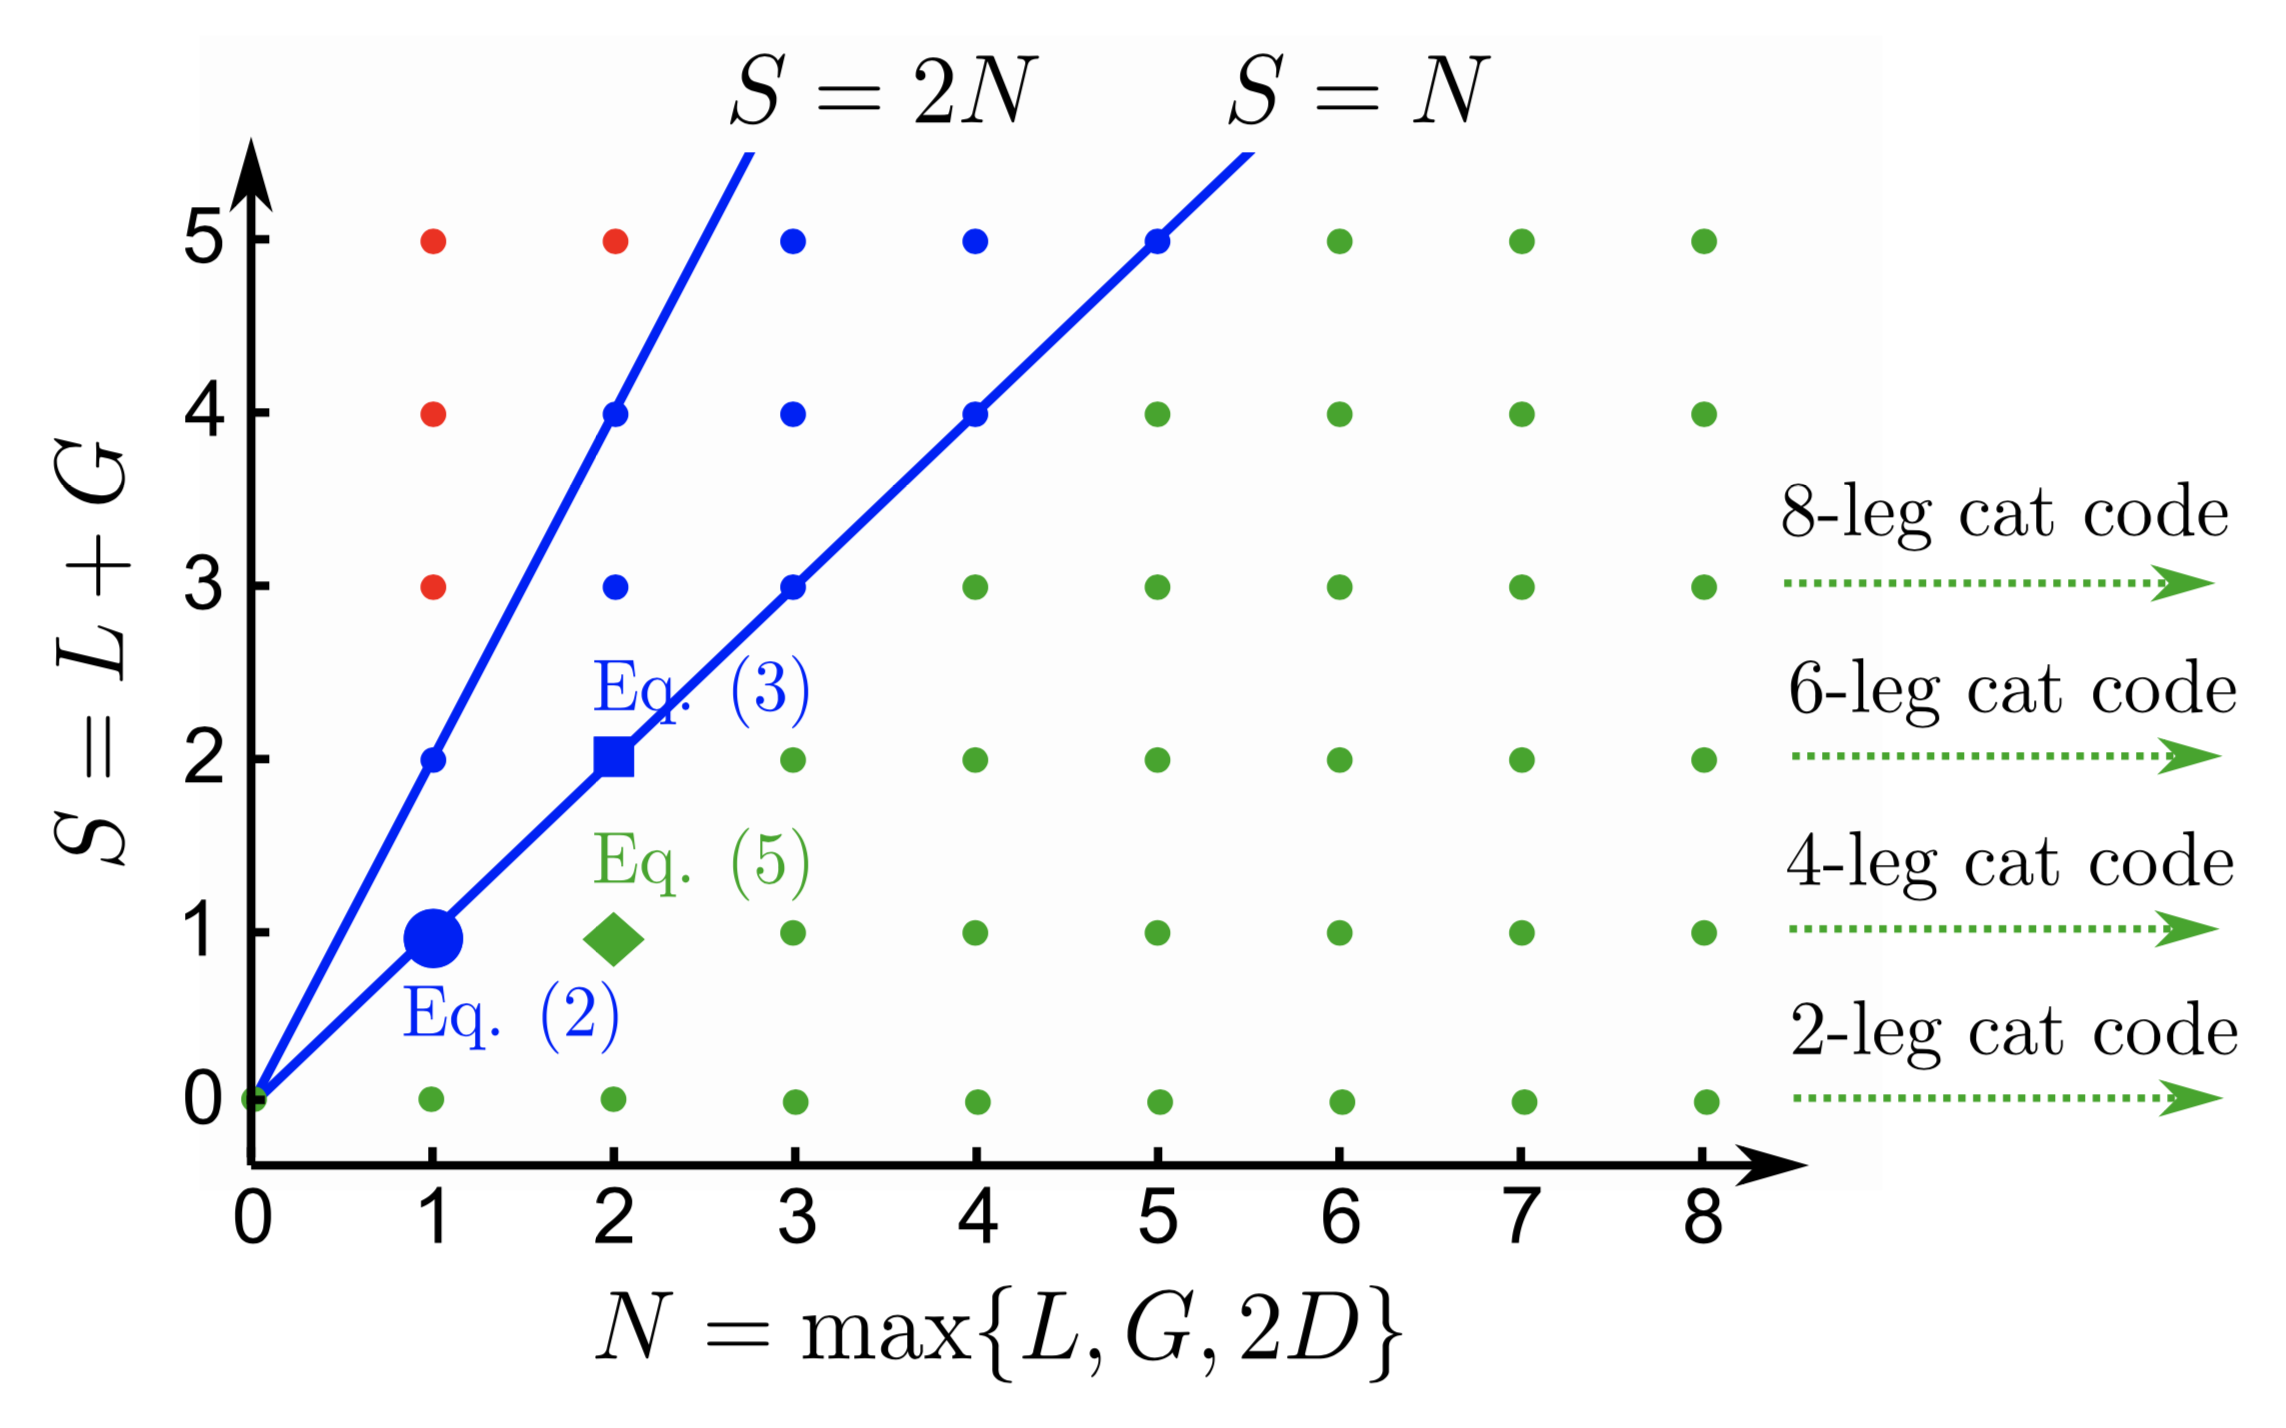
\includegraphics[width=0.5\linewidth,keepaspectratio]{binom_cat.png}	
\caption{Figure borrowed from \cite{michael2016new} comparing binomial codes to cat codes. Observe that, in principle, unlimited dephasing errors can be tolerated by cat codes.}
\end{figure}

\subsection{Performance Comparisons}
\label{sec:perf}

In \cite{albert2017performance}, Albert et al. consider "channel fidelity", $F_\mathcal{E}$,  as numerically tractable proxy for evaluating single-mode bosonic code protection capabilities. The motivation is that the noise model operators are not well behaved whereas optimal recovery for each code can readily be computed by utilizing a semi-definite program when considering channel fidelity. Furthermore, if we assume that our noise is completely described by the lossy bosonic channel (i.e. the encoding, recovery, and decoding are perfect), then channel fidelity essentially describes the robustness of entanglement in the presence of the noisy bosonic channel. Specifically, it is the measure of overlap between the initial state and the final state when considering an initial Bell state such that only the first qubit is acted on by the noise channel.

\begin{figure}[H]
\label{fig:perf}
\centering
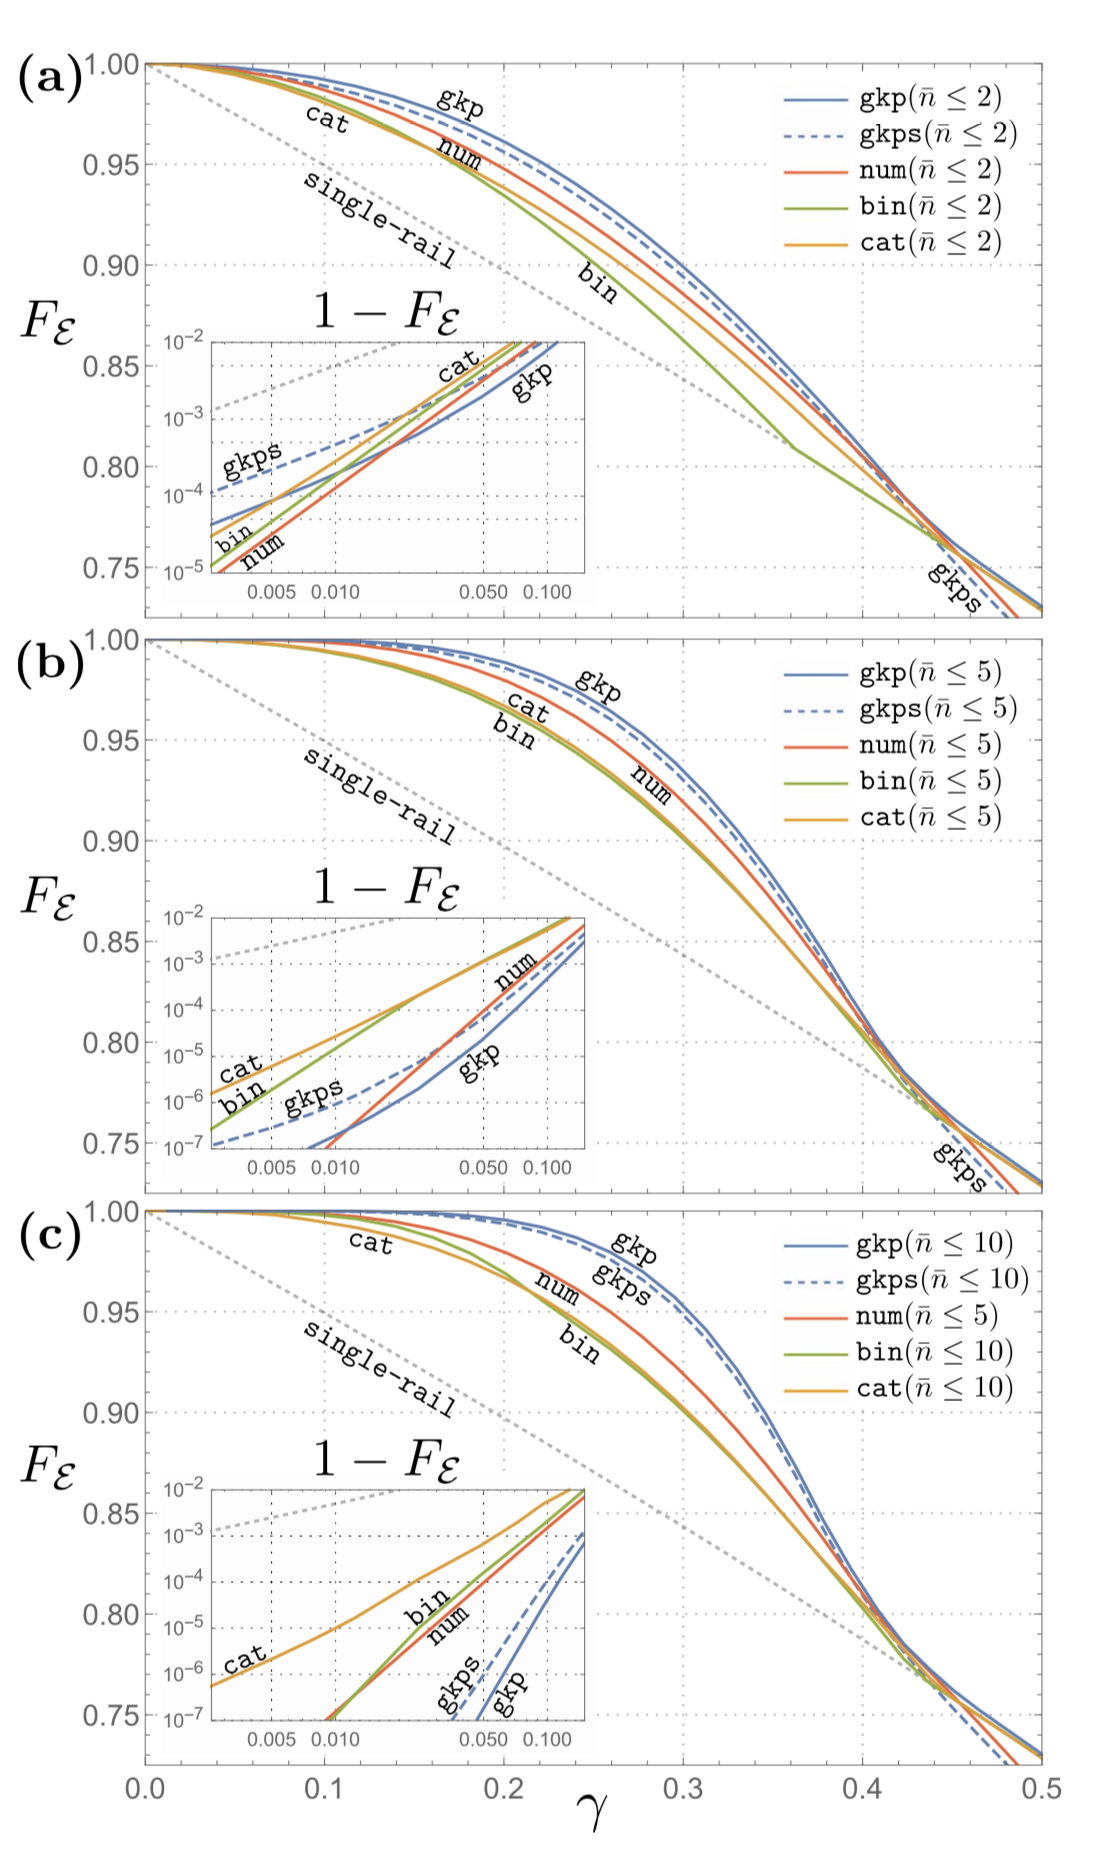
\includegraphics[width=0.5\linewidth,keepaspectratio]{fidelity.png}	
\end{figure}

Figure \ref{fig:perf} summarizes the performance of the optimal code from each family of codes (located by solving the semi-definite program), constraining the mean photon number and varying $\gamma$ (\ref{eq:gamma}).

The numerical results show that codes designed to correct dominant errors at small $\gamma$ do not necessarily lead to good codes at larger $\gamma$. In our case, the cat and binomial codes protect exactly from the first few loss errors by making sure there is adequate Fock state spacing $S$ between the states, as described previously. Both cat and bin allow one to increase $S$ arbitrarily, while gkp codes have $S \in \{0, 1\}$ \cite{albert2017performance}, depending on whether their lattice is shifted from the origin or not. Nevertheless, the gkp strategy of suppressing all errors approximately seems to be the most effective.

Along similar lines, in the paper \cite{noh2018improved} Noh et al. prove that the GKP codes achieve quantum capacity of Gaussian loss channels up to at most a constant gap from an upper bound of the quantum capacity.

\subsection{Multi-Mode Extensions}

Here we briefly summarize recent results based upon these fundamental single-mode codes with the intention of creating near-term physically realizable codes with similar or improved error-correction capabilities.

\subsubsection{Pair-Cat Codes}\label{sec:multi-cat}

The pair-cat codes developed in \cite{albert2018multimode} by Albert et al. opt to use an additional mode not necessarily to improve error-correction capabilities over traditional cat codes (though with greater than two modes this is plausible), but rather to make strides toward physical realizability. In particular, the scheme provides a drastic reduction of the order of the nonlinearity required for realization. 

The code has leading uncorrectable error $\hat{a}\hat{b}$ where $\hat{a}$ and $\hat{b}$ are the loss operators that act on the first and second mode, respectively. Hence, this replaces the uncorrectable error $\hat{a}^2$ for the single-mode cat code, so the code subspaces are of similar quality.

Furthermore, this scheme allows for one to perform discrete QEC techniques (i.e. non-demolition measurement of error syndromes and dynamic control) and continuous QEC techniques (those that don't require active measurement and feedback operations) in parallel which is infeasible in the single-mode case with currently available techniques.

Recall that with cat codes we can use continuous "pumping" to squelch dephasing and discrete photon loss recording to protect from loss. Nevertheless, it turns out that performing both simultaneously is impossible with current techniques \cite{albert2018multimode}. This is related to the fact that the entangling gate for measurement is generated by a cross-Kerr interaction which only commutes with the single-mode jump operator $J_1 \sim \hat{a}^4$ (from equation \ref{eq:single-jump}) at discrete time points. Hence, the dissipation due to $J$ must be turned off during measurement. As it turns out, the fact that the pair-cat code can use photon number difference as opposed to parity as syndrome allows for one to find tune the parameters of the two-mode cross-Kerr interaction to commute with the pair-cat jump operator $J_2 \sim \hat{a}^2\hat{b}^2$.

Furthermore, Albert et al. propose a continuous error correction scheme against loss for the pair-cat codes using Superconducting Nonlinear Asymmetric Inductive eLements (SNAILs)\cite{frattini20173}. These require a lower-order nonlinearity than the array of Josephson junctions required for continuous error correction against photon loss in the single-mode case.

Finally, we observe that $J_2$ spreads out the quartic stabilizing nonlinearity across two modes. This provides the advantage of requiring less photons per mode to have a comparable protection against dephasing and so a slightly lower probability of the leading uncorrectable loss error. Figure \ref{fig:cat} summarizes differences between the codes.

\begin{figure}[h]
\label{fig:cat}
\centering
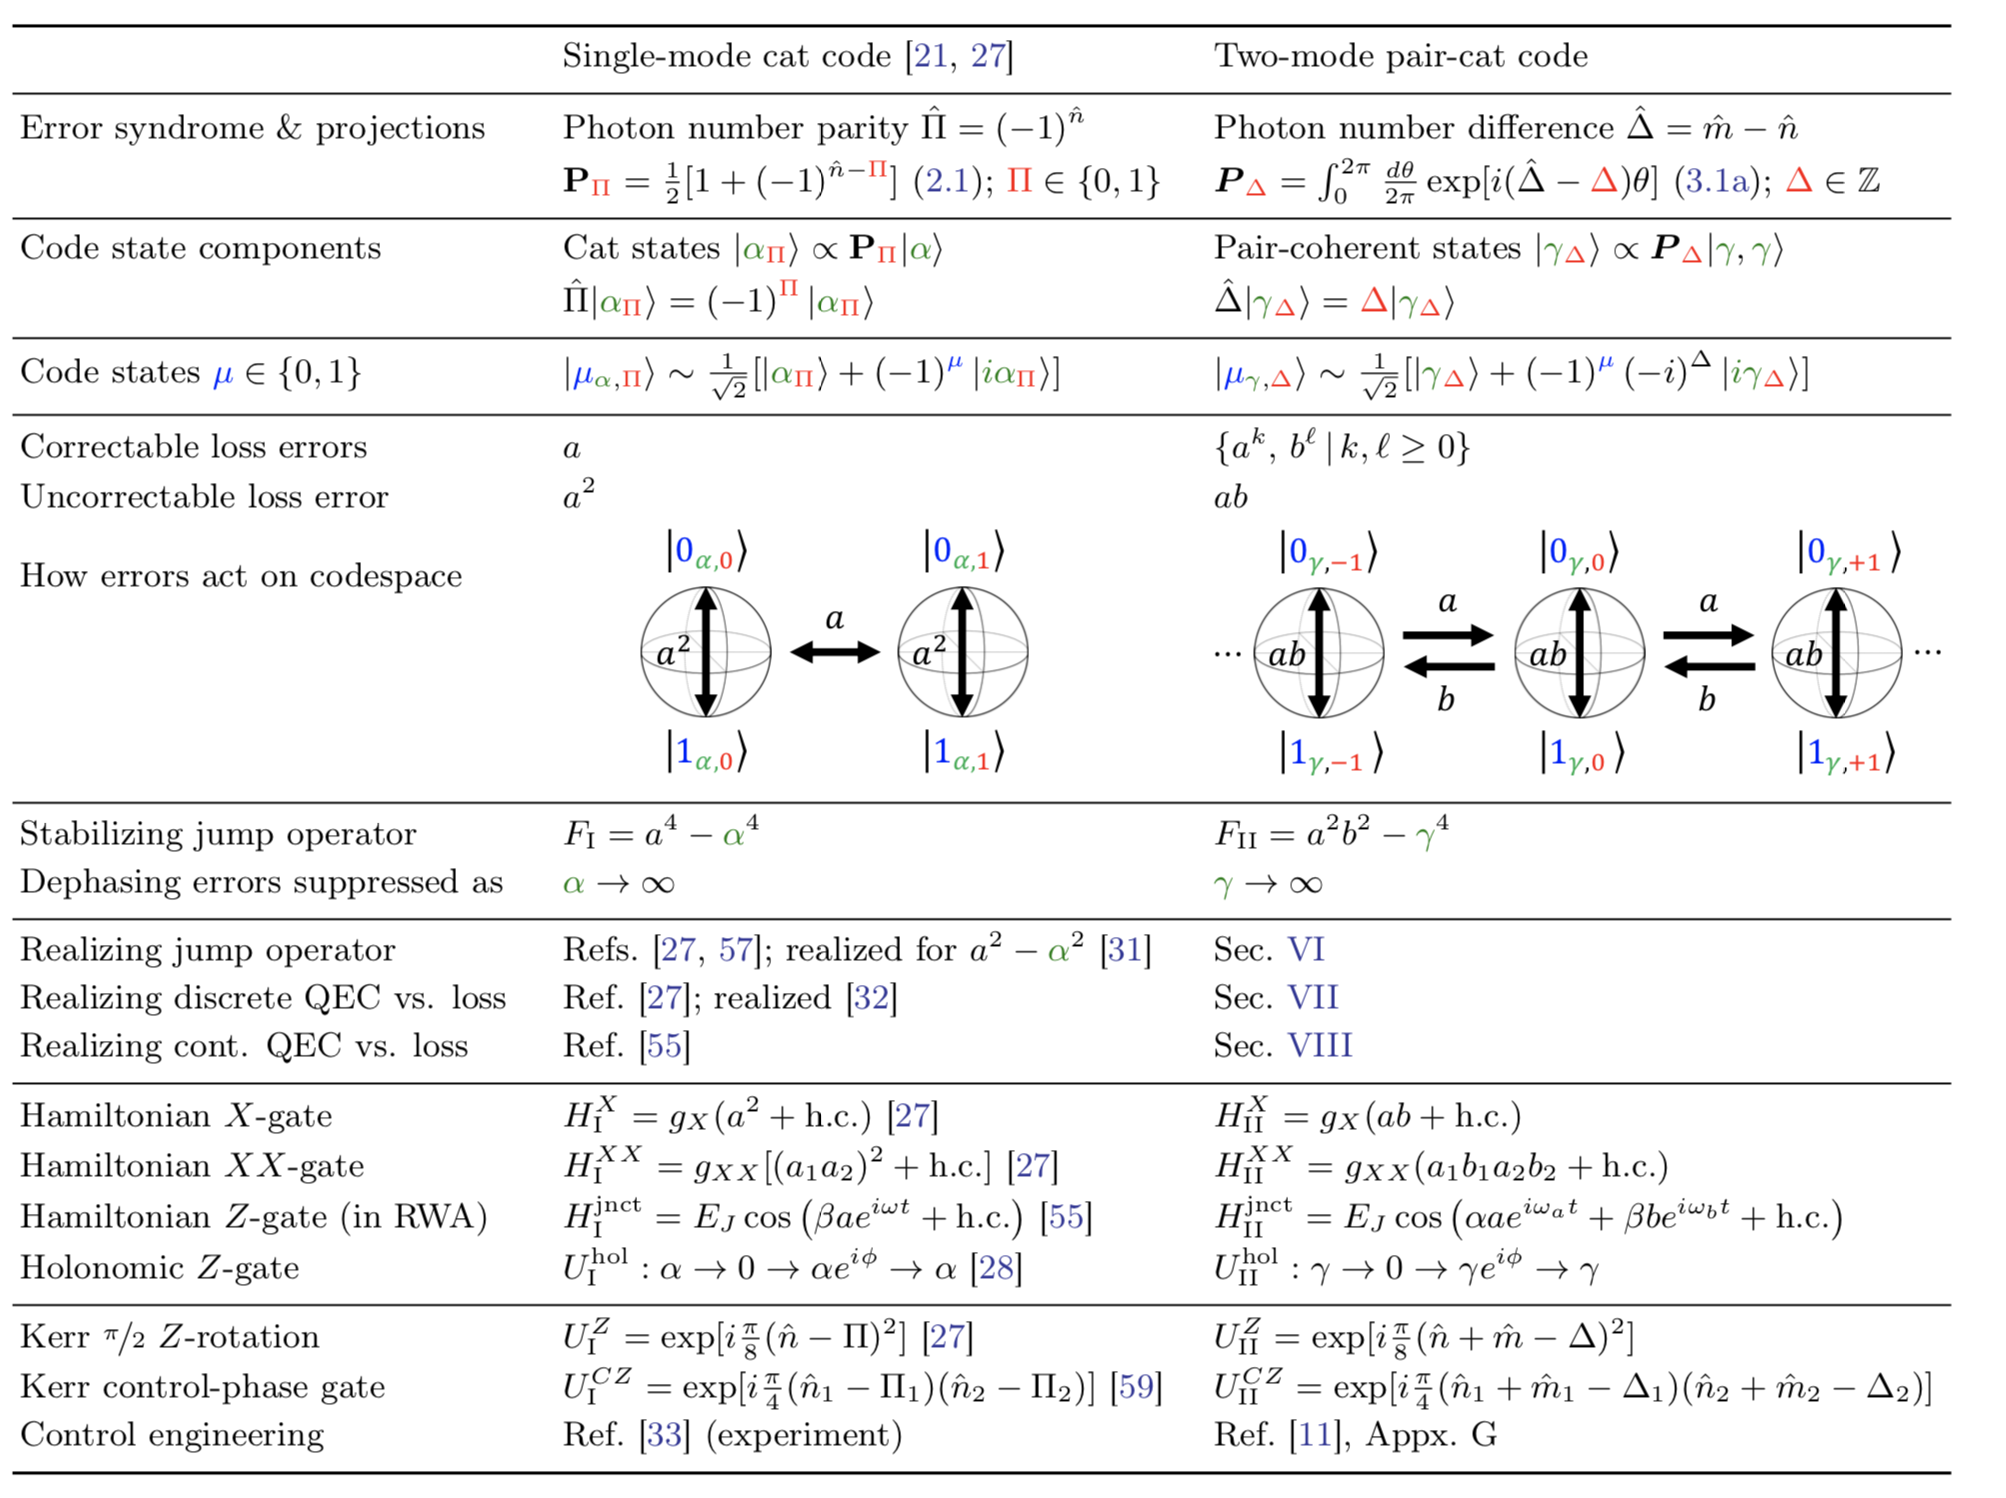
\includegraphics[width=\linewidth,keepaspectratio]{pair_cat.png}	
\caption{Figure from \cite{albert2018multimode} comparing single-mode cat codes to pair-cat codes}
\end{figure}

\subsubsection{$\chi^{(2)}$ Binomial Codes}
\label{sec:multi-binom}

As with pair-cat codes, a motivation for developing a new code is that single-mode cat codes’ universal gate set relies on induced four-wave mixing interactions in Josephson junctions, which are much stronger than optical four-wave mixing in Kerr media. Hence, $\chi^{(2)}$ codes (which are more general than the $\chi^{(2)}$ binomial codes we focus on here) seek to develop quantum computation using only $\chi^{(2)}$ interactions for coherent photon conversion together with linear-optics transformations \cite{niu2018hardware} since it is a lower-order nonlinearity and hence potentially stronger than four-wave mixing.

To build this code Niu et al. establish a symmetry-operator framework that leverages the symmetry of the physical subspace supporting the logical codewords and the symmetry of the measurable syndromes, which we describe below. Ultimately, they show that It is worth emphasizing that the $\chi^{(2)}$ binomial code is the first Fock-basis bosonic QEC code that can correct $N$  photon-loss errors using $O(N)$ photons for its encoding. In fact, all of the codes we have discuss previously require encoding with $O(N^2)$ photons. However, this code requires channel-monitoring resources, which the other studied codes do not, that is used to de-termine the number of photons that have been lost or gained. Hence, this highlights the importance of channel monitoring for the extra error-correction power it can provide.

Now, we consider the notion of "symmetry operators". First, we consider $N$-pump-photon 3-mode subspace $\mathcal{H}_N$ and observe that all states $\ket{\psi} = \sum_{n=0}^N c_n \ket{n, n, N-n} \in \mathcal{H}_N$ obey the following relations

\begin{align}
\begin{split}
	(\hat{n}_s + \hat{n}_p) \ket{\psi} &= N\ket{\psi} \\
	(\hat{n}_i + \hat{n}_p) \ket{\psi} &= N\ket{\psi} \\
	(\hat{n}_s - \hat{n}_i) \ket{\psi} &= 0\ket{\psi}
\end{split}
\end{align}

where $\hat{n}_k \equiv \hat{a}_k^\dag\hat{a}_k$ for each of the three modes $k = s, i, p$. Hence, the photon number parity vector

\begin{align*}
P &= [\hat{n}_s + \hat{n}_i, \hat{n}_s + \hat{n}_p, \hat{n_i + n_p}  ] \mod 2\\
&= [2N, N, N] \mod 2
\end{align*}

is constant $\forall \ket{\psi}$. Motivated by this, we can define symmetry operators 

\begin{align*}
\hat{Z}_{s, p}^{(N + 1)} = \exp(i 2 \pi / (N+1))	\hat{Z}_{s}^{(N + 1)} \otimes \hat{Z}_{p}^{(N + 1)} \\
\hat{Z}_{s, p}^{(N + 1)} = \exp(i 2 \pi / (N+1))	\hat{Z}_{s}^{(N + 1)} \otimes \hat{Z}_{p}^{(N + 1)}
\end{align*}

where

\begin{align*}
\hat{Z}_{k}^{(N + 1)} \equiv \sum_{n=0}^{N}\exp(i 2 \pi n / (N+1))	\ket{n}_k \bra{n}_k
\end{align*}

such that $\ket{n}_k, n \in 0, 1, \cdots, N$ is an $n$-photon Fock state of mode $k, k = s, i, p$.


In order to redundantly encode a lower-dimensional logical basis into a higher-dimensional physical basis, we need additional symmetry operators to stabilize the logical state: within the code’s physical subspace, only the simultaneous unity-eigenvalue eigenstates of all symmetry operators in the given set will be selected as logical-basis states.

In the case of the $\chi^{(2)}$ binomial code, one enforces the physical-subspace symmetry characterized by $\{ \hat{Z}_{s, p}^{(2N)}, \hat{Z}_{s, p}^{(2N)}\}$ above to restrict logical basis states to the subspace $\mathcal{H}_N$. Additionally, to leverage binomial symmetry that will protect the code subspace from distortion by photon loss or gain errors, we introduce the symmetry described by conjugating the photon-number inversion operator with the pseudo-beam-splitter operator. We will not detail this procedure and instead refer you to the original text \cite{niu2018hardware}.

The important aspect we wish to emphasize here is that this symmetry-operator formalism establishes a systematic framework for finding new QEC codes for available measurement schemes and physical subspace choices.

As an example, however, Niu et al. show that when completing the set of symmetry operators, one finds that the simplest case is given by logical states

\begin{align*}
	\ket{B_{\uparrow}} &\sim \ket{0, 0, 3} + \sqrt{3}\ket{2, 2, 1}\\
	\ket{B_{\downarrow}} &\sim \ket{3, 3, 0} + \sqrt{3}\ket{1, 1, 2}
\end{align*}

and one can verify using (\ref{eq:k-l}) that the code is robust against up to second order loss or gain and first order dephasing across all modes.

\subsubsection{Comparisons}

Now, we compare the two multi-mode codes detailed above.

One fundamental difference is that pair-cat codes consist of infinite superpositions of Fock states while $\chi^{(2)}$ codes are finite-dimensional. As a result, only a finite number of photons can be lost for $\chi^{(2)}$ codes while pair-cat codes have a nonzero (albeit exponentially vanishing) probability of losing an arbitrary number of photons. 

We stated that the $\chi^{(2)}$ binomial codes can correct more than one loss if one also knows the total number of photons lost (channel monitoring). Generalized pair-cat codes can introduce a notion of spacing $S$, which we did not detail (but see Section V of \cite{albert2018multimode}), that allows for up to $S$ loss errors in each mode using only knowledge given from error syndromes. Furthermore, it also turns out that pair-cat codes with $S=0$ can detect all loss and gain errors, if we allow three or more mode\cite{albert2018multimode}. This ability is certainly not feasible with the $\chi^{(2)}$ codes.

Nevertheless, the two mode $\chi^{(2)}$ binomial codes can correct dephasing errors $n^l, l \leq N$ exactly, while pair-cat codes correct dephasing approximately.

\section{Conclusion}

\subsection{Importance of Bosonic Systems}

There are many potential advantages to bosonic systems. A clear one is that with each added qubit, several new decoherence channels are added. This multiplies the number of possible errors and requires measuring more error syndromes. Hence, it may be simpler to add physical degrees of freedom using bosonic continuous variable systems. Practically, too, it still seems extremely challenging to build a register of more than on the order of 10 qubits. Hence, bosonic systems may have strong use improving lifetimes of quantum memories.

Past quantum memory, bosonic mode quantum error correction is also useful for quantum teleportation and quantum communication \cite{michael2016new}, which consists of quantum state transfer and generation of high-fidelity entangled pairs of quantum bits between two distant nodes in a quantum network. In \cite{michael2016new} Michael et al. consider a 'pitch-and-catch' scenario for quantum state transfer which can be used for quantum repeaters. They show that simple bosonic codes can greatly increase the fidelity of quantum communication and remote entanglement between hardware modules by being utilized to protect errors from this protocol.

\subsection{Future Developments}

Great strides are still necessary to properly compare the performance of bosonic error correcting codes. Recall the strong assumptions that were made when comparing single-mode codes in Section \ref{sec:perf}: the encoding, recovery, and decoding are perfect and that we can group codes by mean photon occupation number. Furthermore, there are obvious generalizations of this performance analysis to other multi-mode codes. It would be interesting to extend the analysis to two modes to determine the theoretically possible performance of pair-cat codes and $\chi^{(2)}$ binomial codes against photon loss, for example.

Furthermore, we described a symmetry operator framework which provides a systematic way for constructing bosonic QEC codes based on properties of the underlying system dynamics. It also provides a straightforward generalization from qubit-basis three-mode encoding to qudit-basis multi-mode encoding. Hence, we look forward to future works utilizing this formalism.

Additionally, $\chi^{(2)}$ binomial codes seem promising given their efficient usage of photon number ($O(N)$ dependence to correct $O(N)$ loss), but require "channel monitoring" to identify the number of loss errors at a time step. Hence, efficiently performing this monitoring in the hardware is a requirement for this to be a viable code.

The greatest challenge of all, however, seems to be building out hardware efficient for these error correction procedures. Showing that we have the capability of very high fidelity quantum non-demolition measurements of the photon number parity was a breakthrough \cite{sun2014tracking}. As we've seen single-mode codes, such as the cat codes which relied on microwave cavities coupled to Josephson junctions, are being replaced by multi-mode codes which ease the hardware challenge by relying on lower-order nonlinearities which can potentially be corrected by near-term realizable reservoir-engineered microwave cavities \cite{albert2018multimode} or linear optics and $\chi^{(2)}$ interactions.

\nocite{*}
\bibliography{qec_final_project.bib}
\bibliographystyle{amsplain}

\end{document}